\section{Multiplikation $n$-stelliger ganzer Zahlen}

Zuerst müssen wir uns mit dem sogenannten \begriff{Shifting} beschäftigen. Shifting ist ein Vorgang, der das Bitmuster einer Zahl verschiebt. Man unterscheidet 4 Arten des Shifting:
\begin{itemize}
	\item \begriff[Shifting!]{logischer Links-Shift} $\texttt{LSHIFT}_1(a)$: verschiebt das Bitmuster von $a$ um 1 Zeichen nach links, $a_k$ fliegt raus, es werden Nullen eingefügt.
	\item \begriff[Shifting!]{logischer Rechts-Shift} $\texttt{RSHIFT}_1(a)$: verschiebt das Bitmuster von $a$ um 1 Zeichen nach rechts, $a_0$ fliegt raus, es werden Nullen eingefügt.
	\item \begriff[Shifting!]{arithmetischer Links-Shift} $\texttt{ALSHIFT}_1(a)$: verschiebt das Bitmuster von $a$ um 1 Zeichen nach links, $a_k$ fliegt raus, es wird der Wert des rechtesten Bits eingefügt.
	\item \begriff[Shifting!]{arithmetischer Rechts-Shift} $\texttt{ARSHIFT}_1(a)$: verschiebt das Bitmuster von $a$ um 1 Zeichen nach rechts, $a_0$ fliegt raus, es wird der Wert des linkesten Bits eingefügt.
\end{itemize}

Man kann die Multiplikation $a\cdot b$ auch als wiederholte Summation auffassen: $\sum\limits_{i=0}^{n-1} a_i\cdot 2^i\cdot b$. In heutigen Rechnern sind allerdings Addition und Multiplikation gleich schnell. Man kann diese wiederholte Addition aber auch deutlich verbessern:
\begin{itemize}
	\item Gruppe von $k$ Nullen in $a$: sofortiger $\texttt{ARShift}_k(a)$
	\item Gruppe von $k$ Einsen in $a$: $a=[\dots 0\underbrace{\overbrace{1}^{i}\dots\overbrace{1}^{j}}_k0\dots]$. Dann
	\begin{align}
		\sum_{i=j}^{l} 2^i = 2^{l+1}-2^j=2^{j+k}-2^j\notag
	\end{align}
\end{itemize}

Der \begriff{\person{Booth}-Algorithmus} ist eine andere Art der Optimierung. Die Idee ist, dass $a\cdot b$ mit $b=c-d$ $a\cdot b=a\cdot c-a\cdot d$ ergibt. Dazu muss der erste Faktor kodiert werden: Dazu sei $Y=[y_{n-1}\dots y_0]_2$ der zu kodierende Operand. An diesen fügt man eine weitere Stelle $y_{-1}=0$ ein. Der kodierte Operand $Y'=[y'_{n-1}\dots y'_0y_{-1}]_2$ und wir mit $y'_i=y_{i-1}-y_i$ berechnet.

Um den \person{Booth}-Algorithmus zu zeigen, wollen wir $[44]_{10}=[00101100]_2$ mit $[17]_{10}=[00010001]_2$ multiplizieren: \\
\begin{tabularx}{\textwidth}{XXXXXXXXXXXXXXXXX|p{3.2cm}}
	 &
	 &
	\cellcolor{lightgray} & \cellcolor{lightgray} & \cellcolor{lightgray} & \cellcolor{lightgray} & \cellcolor{lightgray} & \cellcolor{lightgray} & \cellcolor{lightgray} &
	\cellcolor{gray} 0 &
	\cellcolor{gray} 0 &
	\cellcolor{gray} 0 &
	\cellcolor{gray} 1 &
	\cellcolor{gray} 0 &
	\cellcolor{gray} 0 &
	\cellcolor{gray} 0 &
	\cellcolor{gray} 1 &
	\tiny 2. Faktor \\
	$\cdot$ &
	 &
	\cellcolor{lightgray} & \cellcolor{lightgray} & \cellcolor{lightgray} & \cellcolor{lightgray} & \cellcolor{lightgray} & \cellcolor{lightgray} & \cellcolor{lightgray} &
	\cellcolor{gray} 0 &
	\cellcolor{gray} 1 &
	\cellcolor{gray} -1 &
	\cellcolor{gray} 1 &
	\cellcolor{gray} 0 &
	\cellcolor{gray} -1 &
	\cellcolor{gray} 0 &
	\cellcolor{gray} 0 &
	\tiny Kodierung 1. Faktor \\
	\hline
	+ &
	&
	\cellcolor{lightgray} 0& \cellcolor{lightgray} 0& \cellcolor{lightgray} 0& \cellcolor{lightgray} 0& \cellcolor{lightgray} 0& \cellcolor{lightgray} 0& \cellcolor{lightgray} 0&
	0 &
	0 &
	0 &
	0 &
	0 &
	0 &
	0 &
	0 &
	\tiny keine Addition \\
	+ &
	&
	\cellcolor{lightgray} 0& \cellcolor{lightgray} 0& \cellcolor{lightgray} 0& \cellcolor{lightgray} 0& \cellcolor{lightgray} 0& \cellcolor{lightgray} 0& 
	0 &
	0 &
	0 &
	0 &
	0 &
	0 &
	0 &
	0 &
	\cellcolor{lightgray} &
	\tiny keine Addition \\
	+ &
	&
	\cellcolor{lightgray} 1& \cellcolor{lightgray} 1& \cellcolor{lightgray} 1& \cellcolor{lightgray} 1& \cellcolor{lightgray} 1&
	1 & 
	1 &
	1 &
	1 &
	1 &
	1 &
	1 &
	1 &
	\cellcolor{lightgray} &
	\cellcolor{lightgray} &
	\tiny 2er Komplement (2. Faktor) \\
	+ &
	&
	\cellcolor{lightgray} 0& \cellcolor{lightgray} 0& \cellcolor{lightgray} 0& \cellcolor{lightgray} 0&
	0 &
	0 & 
	0 &
	0 &
	0 &
	0 &
	0 &
	0 &
	\cellcolor{lightgray} &
	\cellcolor{lightgray} &
	\cellcolor{lightgray} &
	\tiny keine Addition \\
	+ &
	&
	\cellcolor{lightgray} 0& \cellcolor{lightgray} 0& \cellcolor{lightgray} 0&
	0 &
	0 &
	0 & 
	1 &
	0 &
	0 &
	0 &
	1 &
	\cellcolor{lightgray} &
	\cellcolor{lightgray} &
	\cellcolor{lightgray} &
	\cellcolor{lightgray} &
	\tiny 2. Faktor \\
	+ &
	&
	\cellcolor{lightgray} 1& \cellcolor{lightgray} 1&
	1 &
	1 &
	1 &
	1 & 
	1 &
	1 &
	1 &
	1 &
	\cellcolor{lightgray} &
	\cellcolor{lightgray} &
	\cellcolor{lightgray} &
	\cellcolor{lightgray} &
	\cellcolor{lightgray} &
	\tiny 2er Komplement (2. Faktor) \\
	+ &
	&
	\cellcolor{lightgray} 0&
	0 &
	0 &
	0 &
	1 &
	0 & 
	0 &
	0 &
	1 &
	\cellcolor{lightgray} &
	\cellcolor{lightgray} &
	\cellcolor{lightgray} &
	\cellcolor{lightgray} &
	\cellcolor{lightgray} &
	\cellcolor{lightgray} &
	\tiny 2. Faktor \\
	+ &
	&
	0 &
	0 &
	0 &
	0 &
	0 &
	0 & 
	0 &
	0 &
	\cellcolor{lightgray} &
	\cellcolor{lightgray} &
	\cellcolor{lightgray} &
	\cellcolor{lightgray} &
	\cellcolor{lightgray} &
	\cellcolor{lightgray} &
	\cellcolor{lightgray} &
	\tiny keine Addition \\
	\hline
	\cellcolor{lightgray} 1 &
	\cellcolor{lightgray} 0&
	\cellcolor{gray} 0 &
	\cellcolor{gray} 0 &
	\cellcolor{gray} 0 &
	\cellcolor{gray} 0 &
	\cellcolor{gray} 0 &
	\cellcolor{gray} 1 & 
	\cellcolor{gray} 0 &
	\cellcolor{gray} 1 &
	\cellcolor{gray} 1 &
	\cellcolor{gray} 1 &
	\cellcolor{gray} 0 &
	\cellcolor{gray} 1 &
	\cellcolor{gray} 1 &
	\cellcolor{gray} 0 &
	\cellcolor{gray} 0 &
	\tiny Ergebnis ohne Überlauf \\
	\hline
	= &
	 &
	\cellcolor{gray} &
	\cellcolor{gray} &
	\cellcolor{gray} &
	\cellcolor{gray} &
	\cellcolor{gray} &
	\cellcolor{gray} 1 & 
	\cellcolor{gray} 0 &
	\cellcolor{gray} 1 &
	\cellcolor{gray} 1 &
	\cellcolor{gray} 1 &
	\cellcolor{gray} 0 &
	\cellcolor{gray} 1 &
	\cellcolor{gray} 1 &
	\cellcolor{gray} 0 &
	\cellcolor{gray} 0 &
	\tiny Ergebnis mit Überlauf \\
\end{tabularx}

Dazu noch ein paar Bemerkungen:
\begin{itemize}
	\item Statt also mit $[0100000]_2$, $[0001000]_2$ und $[0000100]_2$ zu multiplizieren und die Ergebnisse zu addieren, wird nun also mit $[1000000]_2$, $[0100000]_2$, $[0010000]_2$ und $[0000100]_2$ multipliziert und die Ergebnisse addiert bzw. subtrahiert.
	\item Wie man am Beispiel sieht, kann sich die Anzahl der Additionen auch erhöhen (im Beispiel von 3 auf 4), was aber eigentlich nicht gewünscht ist. Im statistischen Durchschnitt werden im \person{Booth}-Verfahren genauso viele Additionen gebraucht wie ohne \person{Booth}-Verfahren. Der Vorteil liegt aber darin, dass in der Informatik keine Gleichverteilung von Zahlen vorliegt. Vielmehr gibt es häufig Zahlen mit vielen Nullen und durch das Zweierkomplement bei negativen Zahlen häufig viele Einsen am Anfang. Nur durch diese Tatsache hat das \person{Booth}-Verfahren Vorteile gegenüber einer normalen Multiplikation.
	\item Das Verfahren produziert das richtige Ergebnis: $44\cdot 17=[748]_{10}=[1011101100]_2$.
\end{itemize}

Die 3. Möglichkeit die Multiplikation zu verbessern, ist der \begriff{\person{Wallace}-Tree}. Die Idee dahinter ist folgende:
\begin{align}
	\underbrace{\left(\sum_{k=0}^{n} a_k2^k\right)}_{\text{Binärdarstellung }a}\cdot \underbrace{\left(\sum_{k=0}^{n} b_k2^k\right)}_{\text{Binärdarstellung }b} = \sum_{k=0}^{2n}\sum_{i+j=k} a_ib_j2^k\notag
\end{align}

Der \person{Wallace}-Tree-Multiplizierer geht in 3 Schritten vor:
\begin{enumerate}
	\item Berechne für jedes Paar $(i,j)$ mit $1\le i\le n$ und $1\le j\le k$ das Partialprodukt $a_ib_j2^{i+j}$.
	\item Addiere die Resultate dieser Berechnung innerhalb der für den \person{Wallace}-Tree-Multiplizierer spezifischen Baumstruktur stufenweise mithilfe von Voll- und Halbaddierern, bis nur noch 2 Zahlen übrig sind, die addiert werden müssen.
	\item Addiere diese beiden Zahlen mit einem normalen Addierwerk (Carry-Lookahead-Adder).
\end{enumerate}

Der \person{Wallace}-Tree benutzt den Carry-Save-Adder (CSA), der 3 Zahlen addieren kann und 2 Zahlen ausgibt: Die Sequenz der Partialsummen und die Sequenz der Übertragsbits $\to$ 2 gleich lange Zahlen

\begin{figure}[ht]
	\centering
	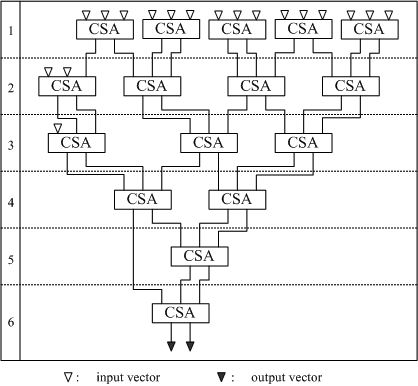
\includegraphics[width=10cm]{images/Wallace-Tree.png}
	\caption{\person{Wallace}-Tree}
\end{figure}

Die Komplexität des \person{Wallace}-Tree ist $T(n)=\mathcal{O}(\log n)$, also in etwa genau so lange wie die Addition!